\section{이론적 배경}

\subsection{천체 관측 시스템}


\subsection{자동초점조절 알고리즘 및 관련 논문 고찰}

이덕규 외(2014)는 복합재 광구조체와 결합하여 전자광학카메라의 영상 품질을 향상시킬 수 있는 초점 조절 장치를 개발하였다.\cite{leedukgu2014}\\
윤종환 외(2011)는 선명도에 관한 기울기를 이용하여 초점이 맞았는지를 확인하는 방법을 사용하였다.\cite{yunjonghwan2011lcd}\\
박석휘 외(2009)는 모바일 폰용 자동 초점 조절 알고리즘을 초점 값 계산 알고리즘을 이용하여 구현하였다.\cite{parksukhui2009Median}\\
이성희 외(1998)는 각 화소들의 미디언 값의 차이를 이용하여 초점을 맞추는 알고리즘을 구현하였다.\cite{leeseonghee1998Median}

\subsection{연구 문제}


\subsection{기존 제품 분석}

Figure \ref{fig:microtouch_3} \가 바로 Micro Touch로, 미국의 Starizona사에서 판매하는 Micro Touch Autofocuser Hand Control system (Wired)이다. 이 제품은 USB 케이블로 컴퓨터와 연결하여 ASCOM 호환 SW에서 제어가 가능하다. 

%%%%%%%새로 그림 추가함 (박기현샘)
\begin{figure}[h]
	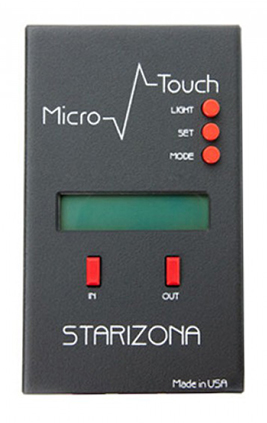
\includegraphics[width=0.6\linewidth]{microtouch_3}
	\caption{Starizona사에서 판매하는 Micro Touch Autofocuser Hand Control system (Wired)}
	\label{fig:microtouch_3}
\end{figure}

%%%%%%%기존에 있던 그림 (박기현샘)
%\begin{wrapfigure}{l}{0.25\textwidth}
%	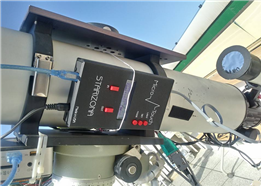
\includegraphics[width=1\linewidth]{telescope1}
%	\caption{Micro Touch가 달린 천체망원경}
%	\label{fig:telescope1}
%\end{wrapfigure}
수가 있다. Fig.2에서 나온 위의 두 버튼(IN, OUT)은 각각 초점을 맞추기 위해 망원경의 길이를 줄이거나 늘일 수 있는 버튼이다. Micro Touch를 수동 혹은 자동으로 작동시켜 IN 또는 OUT의 명령을 내렸을 경우, 모터 초점 조절 장치가 작동하게 된다. 이 모터 초점 조절 장치는 모터를 움직여 천체망원경의 경통의 길이를 조절할 수 있도록 한다. 경통의 길이가 변화하면 그에 따라서 빛이 퍼지는 정도가 달라지므로 이를 잘 조정하면 망원경으로 관측하는 천체의 초점을 맞출 수 있다.

\subsection{컨트롤러 결정}

\begin{wrapfigure}{l}{0.05\textwidth}
	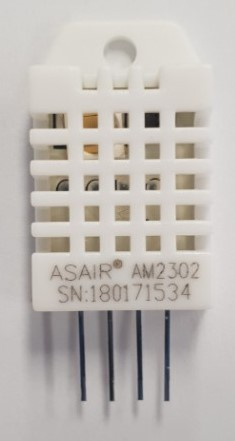
\includegraphics[width=1\linewidth]{DHT22}
	\caption{DHT22}
	\label{fig:DHT22}
\end{wrapfigure}
이 연구를 진행하는 데 Arduino를 사용하는 것이 가장 기본이라고 판단하였기 때문에 Arduino로 실행할 수 있는 것 중 쉬운 축이라고 생각되는 온습도 감지기(DHT22)를 활용하여 온습도를 측정하는 일이었다. 기판을 짜고 코드를 입력하면 Serial Monitor에 온도와 습도가 delay 함수에서 지정한 만큼의 간격을 두고 계속 출력된다. 이를 응용하여 OLED(OLED1306)에 온도와 습도를 실시간으로 출력하는 프로그램을 만들 수도 있다.

\subsection{스테핑 모터}

\subsubsection{스테핑 모터의 종류}

아래 기사 참고할 것 (박기현샘)
http://www.motioncontrol.co.kr/default/news/?nwsid=n3&uid=5002
%%
스테핑 모터의 종류는 크게 bipolar와 unipolar 타입으로 나눌 수 있다. 하나는 2상 6선식이라고 불리는 bipolar 스테핑 모터로, 전선이 6개가 연결되어 있다. 2상 4선식이라고도 불리는 unipolar 타입은 전선이 4개가 연결된 모터로, 구동 방식은 bipolar 타입과 크게 다르지 않다.\\
본 논문에서 사용된 스테핑 모터는 2상 6선식 모터이지만, 그 구동 방식이 비슷하므로 bipolar 스테핑 모터에서 필요 없는 2번 선과 5번 선을 제거하는 것으로 bipolar 스테핑 모터를 unipolar 스테핑 모터처럼 구동할 수 있다.

\subsubsection{스테핑 모터의 작동 원리}

\begin{wrapfigure}{l}{0.5\textwidth}
	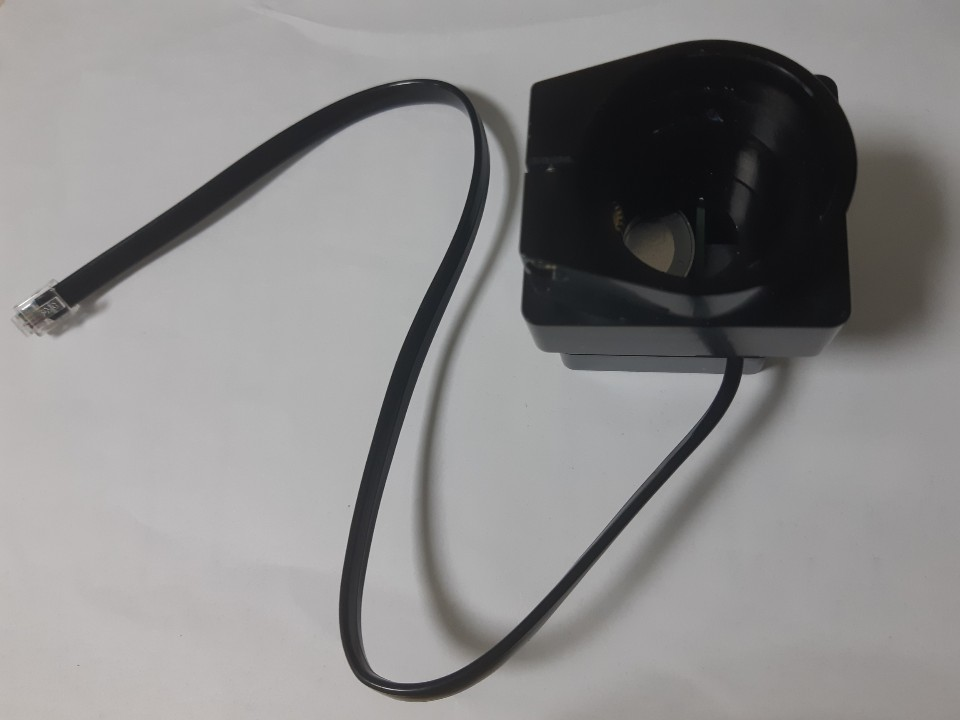
\includegraphics[width=1\linewidth]{stepmotor}
	\caption{스테핑 모터}
	\label{fig:stepmotor}
\end{wrapfigure}
우리가 실생활에서 볼 수 있는 모터 대부분은, 예를 들어 선풍기의 모터는, DC모터이다. DC모터는 전류가 흐르는 상태에서는 계속 회전하기 때문에 원하는 위치에서 멈추는 것이 어렵다. 하지만 스테핑 모터는 회전자 주위에 여러 고정자가 존재하여, 이 고정자들에 흐르는 전류의 변화량에 따라서 회전자 내부의 자석을 회전시키기 때문에, 전류의 양에 따라서 일정한 각도를 정확하게 회전시킬 수 있다. 따라서 본 연구와 같이 회전시키는 것이 중심이 아닌, 정확하게 얼마나 돌아갔는지(어느 각도만큼 돌아갔는지가 중요하게 작용할 때) 대부분 스테핑 모터를 활용하고는 한다. 이렇듯 선별로 흐르는 전류의 양에 의해 회전하는 정도와 속도를 결정할 수 있기에 흔히 ‘마이크로 스테핑’을 이용하여 전류를 여러 단계로 나누어 흘려보내어 더 정밀하게 모터를 제어하는 방법들도 존재한다. 대부분의 스테핑 모터는 1 스텝당(full step) 1.8도를 돈다고 알려져 있다.


